% 02.06.2016 12:00 CET last changed by a.holzinger
% General Template for LNCS and LNAI contributions based on llncs, adapted by ah
% Many thanks to the TRS team
% In case of using eps compile via 1) TeXify and then proceed with 2) dvi2pdf
%
\documentclass{llncs}
\usepackage{float}

\usepackage[dvips]{graphicx}
\usepackage[ruled,vlined]{algorithm2e}
\usepackage{amsfonts}
\usepackage{amssymb}
\usepackage{amsmath}
\usepackage{mathtools}

\providecommand{\abs}[1]{\lvert#1\rvert}
\providecommand{\norm}[1]{\lVert#1\rVert}

\usepackage{calc}
\usepackage{subfigure}

\usepackage{color}
\usepackage{soul}
\usepackage{comment}

\usepackage[font=small, labelfont=bf]{caption}

\newtheorem{prop}{Property}

\newenvironment{Bitemize}{\renewcommand\labelitemi{\textbullet}\begin{itemize}}{\end{itemize}}

\begin{document}

\title{The more the merrier - Federated learning from graph based recommendations}

% \author{Bernd Malle\inst{1}\inst{2}, Peter Kieseberg\inst{1}\inst{2}, Edgar Weippl\inst{2}, Andreas Holzinger\inst{1}}

%\institute{Holzinger Group HCI-KDD \\
%Institute for Medical Informatics, Statistics \& Documentation\\
%            Medical University Graz, Austria\\
%            \texttt{b.malle@hci-kdd.org}
%\and
%SBA Research gGmbH, Favoritenstraße 16, 1040 Wien \\
%			\texttt{PKieseberg@sba-research.org}
%}
	
\maketitle

% ==================================
%				ABSTRACT
% ==================================
\begin{abstract}
	
With Google's \textit{Federated Learning} \& Facebook's introduction of client-side NLP into their chat service, the era of client-side Machine Learning has finally begun. While interesting ML approaches beyond the realm of toy examples were hitherto confined to large data-centers and powerful GPU's, exponential trends in computing technology and the introduction of billions of smartphones bring sophisticated processing pipelines within reach of even hand-held devices. Such approaches hold several promises: 1. Without the need for powerful server infrastructures, even small companies could be scalable to millions of users easily and cost-efficiently; 2. Since data only used in the learning process never need to leave the client, personal information can be used free of privacy and data security concerns; 3. Since privacy is preserved automatically, the full range of personal information on the client device can be utilized for learning; and 4. without round-trips to the server, results like recommendations can be made available to users much faster, resulting in enhanced user experience. In this paper we propose an architecture for federated learning from personalized, graph based recommendations computed on client devices, collectively creating \& enhancing a global knowledge graph. In this network, individual users will 'train' their local recommender engines, while a server-based voting mechanism aggregates the developing client-side models, preventing over-fitting on highly subjective data from tarnishing the global model.

\medskip

\textbf{Keywords}: machine learning, federated learning, interactive learning, the local sphere, graph based recommendations, personalized ML models, distributed bagging


\end{abstract}

\renewcommand{\thesubfigure}{\thefigure.\arabic{subfigure}}
\makeatletter
\renewcommand{\p@subfigure}{}
\renewcommand{\@thesubfigure}{\thesubfigure:\hskip\subfiglabelskip}
\makeatother


% ==================================
%			INTRODCUTION
% ==================================
\section{Introduction and Motivation}
\label{sect:intro_motivation}

A 2006 paper \cite{leskovec2006recpatterns} examined recommender networks crystallizing from purchases based upon previously received product recommendations by employing an online shopping system observing purchases and recommendations of several product categories. Users of the platform were modeled as nodes in a graph with recommendations connecting them. This resulted in a collection of fragmented subgraphs representing series of so called \textit{recommendation cascades}. Their analysis revealed that about 95\% of all relevant recommendations originated from a subgraph with a diameter of only ~1.2, that is a node's immediate vicinity. Similar findings were also reported from the blogosphere \cite{leskovec2007blogpatterns}.

Observing a seemingly unrelated field of Software Development, the early 2010s have yielded new Web frameworks bringing the power of publish/subscribe systems within reach of even single developers. These mechanisms work by reconciling two potentially conflicting interests in a set-theoretic way: The set of all data-points a client wishes to receive are intersected with the set of all data-points a server is allowed to publish to specific individuals. This intersection is then pushed down to the client and constantly kept up to date, obviating the need for a client to permanently send new data / update requests. This leads to a certain sub-sample of global data permanently residing on the client device; in the case of a graph structure (social network, knowledge graph) this sub-sample would (at least) contain a node's immediate neighborhood.

Combining these two developments, we arrived at the definition of a \textit{local sphere} residing on a client device, representing a subset of the globally available information within a system. As for most recommendations those data points are seemingly the only ones relevant, we conjecture a new system architecture based on client-side, graph-based recommenders whose interaction with the user results in modifications of the local sphere, which by means of publish/subscribe are subsequently propagated throughout the system.

We therefore challenge the traditional notion of Machine Learning as happening on powerful, centralized servers and would like to replace them by a collective of mundane personal devices. Although this might seem futuristic, we see it as a logical solution especially to the problems of large-scale graph analysis \cite{leskovec2006samplinggraphs} as well as a continuation of a long-running trend towards employing commodity hardware for even the most demanding applications \cite{al2008scalable}.


\begin{figure}[H]
	\begin{center}
		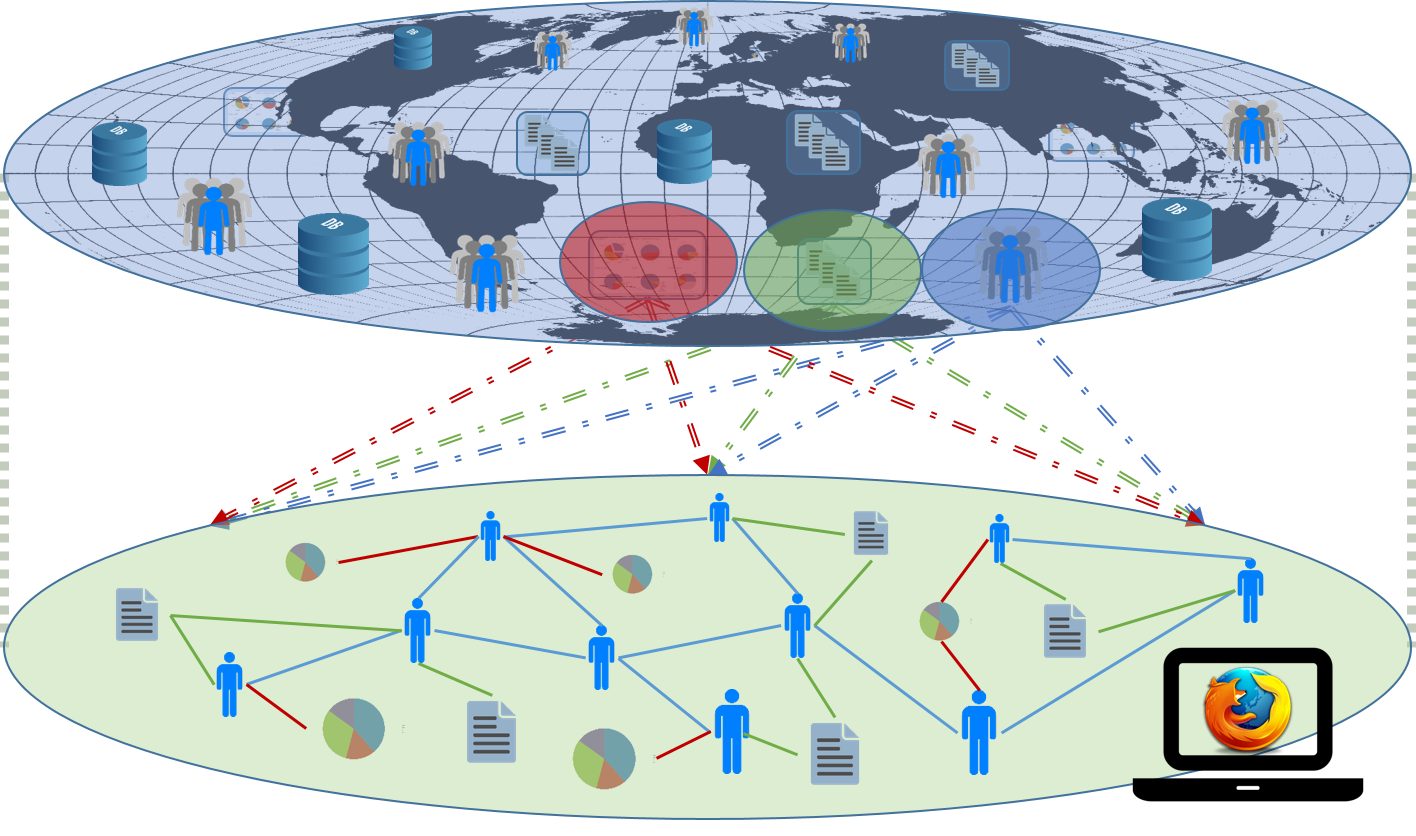
\includegraphics[width=0.8\textwidth]{figures/local_sphere}
		\caption{Publish-subscribe mechanism used by a client to constantly synchronize a subsample of a \textit{global database} to constitute what we term the \textit{local sphere}. Note that the local sphere is a superset of the user's data - it may contain items a user is not actually requesting, but might be significant for computing relevant recommendations.}
		\label{fig:local_sphere}
	\end{center}
\end{figure}



\section{Theoretical building blocks}
\label{sect:bg_related}

Four building blocks


\subsection{Client-side Machine Learning}
\label{ssect:cs_ML}

\cite{2003automaticKEfromWebDocuments}
\cite{mcmahan2016communication}
\cite{konevcny2016federatedlearning}
\cite{konevcny2016federatedoptimization}
\cite{2017secureaggregation}

\cite{shi2012reciprocalrank}

\subsection{Privacy \& Security}
\label{ssect:privacy_security}

\cite{malle2016right}

\subsection{interactive Machine Learning (iML)}
\label{ssect:iML}

\cite{2016iMLExperiment}
\cite{2016HolzingeriML}
\cite{2016KiesebergDITL}

\subsection{distributed Bagging}
\label{ssect:dist_bag}

\cite{breiman1996bagging}

\begin{figure}[H]
	\begin{center}
		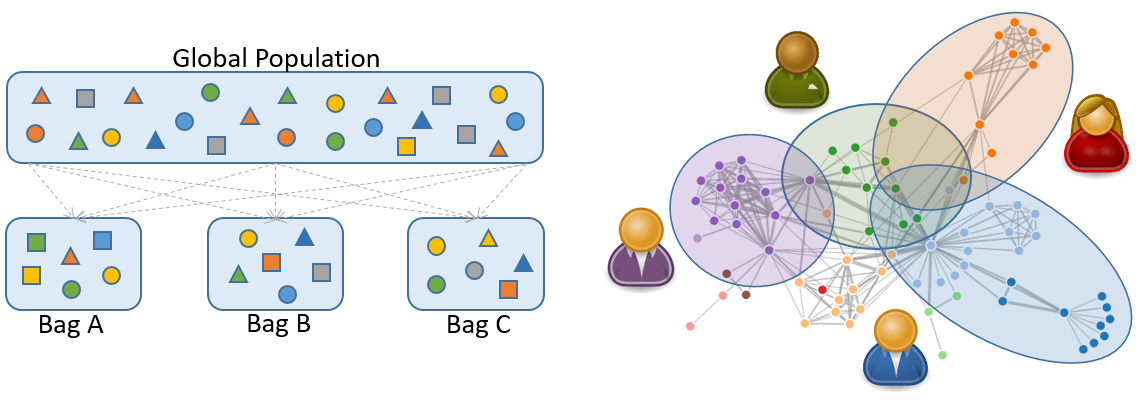
\includegraphics[width=1\textwidth]{figures/bagging_vs_local_sphere}
		\caption{Bagging vs. Spheres: To the left we depict the traditional bootstrap approach. To the right we see a global graph with user-defined \textit{local spheres}, which influence each other via their overlapping segments (albeit each residing on their respective client). The graph was generated using D3.js \cite{zhu2013d3js}}
		\label{fig:bagging_vs_sphere}
	\end{center}
\end{figure}


\section{Proposed Workflow}
\label{sect:workflow}

In order to organize a perfect interplay of the components described above, we suggest the following sequence of interactions between the server (global sphere), client (local sphere), user (actually relevant data plus secure personal information) as well as the 'world' (all the information available on the Web or specialized online services):

\begin{enumerate}
	\item The client defines a subscription for all data which might interest the user.
	\item The server computes a local sphere by reconciling the client's request with it's own security / publication policy and pushes it down to the client.
	\item Once the local sphere is instantiated, the actually relevant user data are prepared \& visualized; the whole local sphere is instantiated within a client-side graph library in the background.
	\item Client-side recommender algorithms continuously check the local sphere that is not already part of the user data for possible new information and recommend them on occasion.
	\item Client-side 'providers' utilize the users personal information accessible via her local device or social media account, scanning the web for suitable information items on every user interaction with the local sphere. Such information items are again recommended to the user on a regular basis.
	\item The user interacts with her data via adding, connecting or re-arranging items. Each time new information is introduced into a local sphere it is synchronized to the server and - via it's overlapping segments with other local spheres - to those respective clients as well.
\end{enumerate}

As a consequence of this interactive workflow, it might even be possible to renounce the idea of a centrally curated global graph demanding tremendous computational power, energy as well as financial resources. Apart from occasional server-side sampling for reasons of security and general prudence, a global graph would emerge, be sustained and developed purely through the growth and / or modification of all the local spheres that fabricate it.


\section{Conclusion}
\label{sect:conclusion}

In this paper, we have welcomed the era of client-side machine learning and introduced the concept of the \textit{local sphere} as a logical building block for future collective (or federated) machine learning systems. We have derived the local sphere idea for graph-based recommendations from earlier works and defined the 4 theoretical building blocks of our proposed system, describing the advantage each of their underlying approaches contributes to the system. Finally, we presented a possible workflow architecture which would allow a global graph to exist entirely as an abstract, logical layer on top of a multitude of local sphere's interaction with one another and the rest of the world.

\newpage

\bibliographystyle{unsrt}
\bibliography{references}

\end{document}
